% Overleaf: https://www.overleaf.com/9984419175fbspjppxpygz
% (The final document with the correct format is the Overleaf one)

\RequirePackage[2020-02-02]{latexrelease}
\documentclass[twocolumn]{revtex4}

\usepackage[catalan]{babel}
\renewcommand\acknowledgmentsname{Agraïments}

\usepackage[utf8]{inputenc}
\usepackage{lmodern}
\usepackage[T1]{fontenc}
\usepackage{mathtools}
\usepackage{float}
%\usepackage{multicol}
\usepackage{csvsimple}
\providecommand{\abs}[1]{\lvert#1\rvert}
\usepackage{braket}
\providecommand{\eq}[2]{
    \begin{equation}
        #2
    \label{eq:#1}
    \end{equation}
}
\providecommand{\eqgat}[2]{
    \begin{gather}
        #2
    \label{eq:#1}
    \end{gather}
}
\usepackage{amsmath}
\usepackage{amsfonts}
\DeclareMathOperator{\calH}{\mathcal{H}}
\DeclareMathOperator{\calL}{\mathcal{L}}
\DeclareMathOperator{\calN}{\mathcal{N}}
\DeclareMathOperator{\calO}{\mathcal{O}}
\DeclareMathOperator{\tr}{tr}
\usepackage{fancyhdr}
\usepackage{wrapfig}
\usepackage{graphicx}
\usepackage[hidelinks]{hyperref}


\begin{document}


\pagestyle{fancy}
\lhead{\bf Entropia d'entrellaçament i holografia}
\rhead{Ferran Rodríguez Mascaró}
\lfoot{Treball de Fi de Grau}
\rfoot{Barcelona, Juny 2023}


\title{Entropia d'entrellaçament i holografia}
\author{Autor: Ferran Rodríguez Mascaró}
\email[Adreça electrònica: ]{ferran.r.m11@gmail.com} %optional
\affiliation{Facultat de F\'{\i}sica, Universitat de Barcelona, Diagonal 645, 08028 Barcelona, Spain.}
\author{Tutor: Dr. Pablo Bueno Gómez}
%\date{\today}


\begin{abstract}
    {\bf Resum:} La correspondència AdS/CFT, també anomenada \emph{holografia}, és una dualitat física entre teories de gravetat quàntica en espaitemps d'anti-de Sitter (AdS) i certes teories quàntiques de camps (QFTs) amb simetria conforma definides en la frontera d'aquests espais. L'anomenat diccionari hologràfic descriu com quantitats de cadascuna d'aquestes teories es poden traduir en quantitats de l'altra. Una magnitud important del diccionari hologràfic és l'entropia d'entrellaçament (EE) de regions de la frontera, que mesura el grau d'entrellaçament quàntic entre aquestes regions i els seus complementaris. En aquest treball, estudiem diferents aspectes de l'EE en el context hologràfic. Després d'una revisió d'AdS/CFT i aspectes generals de l'EE a QFT, introduïm la fórmula de Ryu-Takayanagi, que calcula l'EE hologràfica de regions a la frontera en el límit semiclàssic de la part gravitacional de la dualitat. Duem a terme càlculs explícits i comprovacions generals de la fórmula, revisem les seves generalitzacions en considerar correccions cordoses i quàntiques, i comentem la seva relació amb la termodinàmica dels forats negres i l'aflorament de dinàmiques gravitacionals.
\end{abstract}


\maketitle


\section{Introduction} \label{s:Intro}
La cerca per una unificació de teories quàntiques i la gravetat és un repte de la física teòrica que fa molt temps que dura. La correspondència AdS/CFT ---sorgida a finals dels 1990s en el context de la teoria de cordes \cite{maldacena_large_1999}--- proveeix aquesta unificació en el cas particular d'espaitemps amb una frontera de tipus temps. AdS/CFT és també una materialització del principi hologràfic, que estableix que teories de gravetat quàntica han d'admetre una descripció equivalent en termes de teories que viuen a la frontera dels seus espaitemps.
A més de les seves implicacions fonamentals en la cerca d'una teoria definitiva de totes les interaccions, AdS/CFT proveeix un marc de treball útil per provar aspectes de teories quàntiques de camps (QFTs) en règims en els quals les eines usuals no es poden aplicar ---{\emph e.g.,} quan els camps estan fortament acoblats--- usant les eines de la relativitat general.
Addicionalment, AdS/CFT ens permet estudiar el comportament quàntic de la gravetat relacionant-la amb QFTs ben definides i ben enteses.
En aquest treball estudiem un exemple del primer tipus d'aplicacions, concretament, com l'entrellaçament quàntic de regions d'algebres en QFTs hologràfiques es codifica en una quantitat completament clàssica de la banda gravitacional.

En la secció \ref{s:Holo_AdS/CFT} introduïm el principi hologràfic i la correspondència AdS/CFT. La noció d'entropia d'entrellaçament (EE) i algunes de les seves propietats ---incloent una generalització de la primera llei de la termodinàmica--- en el context de les teories de camps conformes (CFTs) es presenten en la secció \ref{s:EE_CFT}. En la secció \ref{s:EE_Holo} introduïm la fórmula de Ryu-Takayanagi, que ens permet calcular l'EE hologràfica de regions de la frontera a partir de l'àrea de funcions extremals en l'espai d'anti-de Sitter (AdS). Calculem explícitament l'EE en el cas d'una regió circular en CFT$_3$ i verifiquem que el model compleix la propietat fonamental de la subadditivitat forta. A més, proveïm un resum de com la fórmula de Ryu-Takayanagi es corregeix amb efectes cordosos i quàntics.


\section{Holografia i AdS/CFT} \label{s:Holo_AdS/CFT}


\subsection{El principi hologràfic} \label{ss:Holography}

Donada una regió finita d'espai, imaginem un procés pel qual se li afegeix matèria de forma contínua. Això farà que l'entropia augmenti. Però, hi ha un límit en la quantitat de matèria que es pot afegir a la regió, que correspon al moment en què formem un forat negre. L'entropia d'un forat negre només depèn de l'àrea de la seva superfície, i es defineix com \cite{bekenstein_black_1973}
\eq{BH}{
    S_\text{BH} = \frac{ A_\text{H} }{ 4 G } \ ,
}
en unitats de Planck, on $A_\text{H}$ és l'àrea de l'horitzó de successos del forat negre i $G$ és la constant gravitatòria de Newton. Per tant, l'entropia màxima que una regió pot contenir és definida per la seva àrea dividida per $4G$.

Això implica que els graus de llibertat dins d'una certa regió creixen amb l'àrea de la frontera i no amb el volum de la regió, com un podria esperar. Això porta al \emph{principi hologràfic}, que diu que en una teoria de gravetat quàntica tots els fenòmens físics dins d'un cert volum han de ser descrits en termes d'una teoria definida en la frontera d'aquesta regió \cite{t_hooft_dimensional_2009}.


\subsection{Correspondència AdS/CFT} \label{ss:AdS/CFT}

La \emph{correspondència AdS/CFT}, alguns cops anomenada simplement \emph{holografia} o \emph{dualitat gauge-gravetat} \cite{maldacena_large_1999}, és una materialització explícita del principi hologràfic. Estableix l'equivalència física completa entre teories de gravetat quàntica que viuen en espaitemps d'AdS i certs tipus de CFTs que viuen en la frontera d'aquests espaitemps. Si la teoria gravitacional es defineix en $(d+1)$ dimensions espaitemporals, la CFT dual es defineix en $d$ dimensions espaitemporals i, de forma rigurosa, la teoria gravitacional serà un ''holograma'' de la CFT. AdS/CFT ens permet estudiar aspectes de cadascuna d'aquestes teories a partir de l'altra. L'anomenat \emph{diccionari hologràfic} mapeja quantitats (observables) entre les teories gravitacionals i les seves CFTs duals \cite{witten_anti_1998}. Per exemple, un espaitemps d'AdS buit sense matèria és dual a l'estat del buit de la CFT, i un espaitemps d'AdS amb un forat negre dins es correspon a un estat termalitzat en la CFT.

Un \emph{espaitemps d'anti-de Sitter} és un espaitemps maximalment simètric amb curvatura negativa, solució de les equacions de camp d'Einstein amb constant cosmològica negativa. La mètrica d'un espaitemps d'AdS de $(d+1)$ dimensions en coordenades de Poincaré és
\eq{AdS_PP-metric}{
\mathrm{d} s_{\text{AdS}_{(d+1)}}^2 = \frac{L^2}{z^2} \left( -\mathrm{d} t^2 + \mathrm{d} z^2 + \sum_{i=1}^{d-1} \mathrm{d} x_i^2 \right) \ ,
}
on el temps i les dimensions temporals $t , x_i \in (-\infty,+\infty)$, una dimensió extra $z \in (0,+\infty)$ alguns cops anomenada \emph{coordenada hologràfica}, i on $L$ és el \emph{radi d'AdS}. Fixant la coordenada $z$, la mètrica es redueix a la d'un espaitemps de Minkowski $d$-dimensional ``pesat'' pel factor $1/z^2$. Per tant, AdS es pot laminar en espaitemps de Minkowski que viuen a diferents valors de $z$.

\begin{wrapfigure}[13]{r}{0.25\textwidth}
\centering
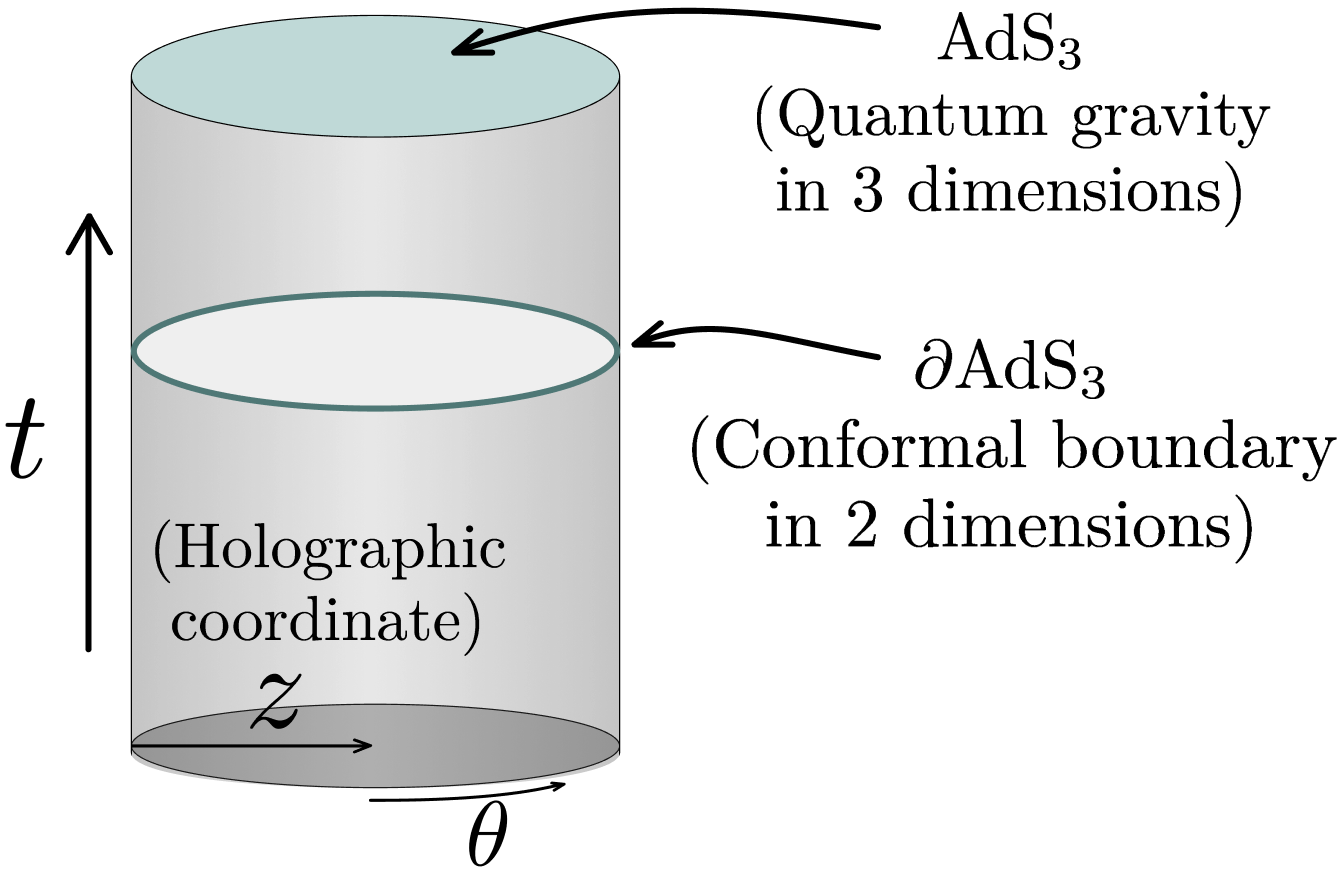
\includegraphics[width=0.25\textwidth]{../../Imatges/AdS_Cylindric.png}
\caption{Espaitemps d'AdS$_3$. En la frontera conforma és on viu la CFT$_2$.}
\label{fig:AdS}
\end{wrapfigure}

AdS$_{d+1}$ es pot representar com un cilindre on cada llesca correspon a un temps constant i on $z$ creix radialment cap al centre \cite{hawking_large_2008}. Cada llesca té una frontera $d$-dimensional $\partial$AdS$_{(d+1)}$ on hi viu la CFT$_d$ (Fig.~\ref{fig:AdS}).

Les \emph{teories de camps conformes}, per altra banda, són QFTs que són invariants sota transformacions conformes. Aquestes són transformacions que preserven els angles i que deixen la mètrica invariant fins a un factor global \cite{di_francesco_conformal_1997}. El grup de Poincaré és un subgrup del grup conforme, però hi ha transformacions addicionals corresponents a les dilatacions i a transformacions conformes especials. El nombre de generadors d'una CFT $d$-dimensional coincideix amb el nombre d'isometries d'un espaitemps d'AdS $(d+1)$-dimensional. Aquesta és una insinuació de la dualitat hologràfica.

El primer cas de correspondència AdS/CFT descrita va ser la dualitat entre la teoria $d=4$, $\calN=4$ de Super Yang-Mills i la teoria de camps de tipus-IIB en AdS$_5 \times $S$_5$ \cite{maldacena_large_1999}, però diversos altres exemples són coneguts actualment. Vàries normes generals de la dualitat poden ser explotades sense especificar el contingut complet de les teories, i aquí ho utilitzarem.

AdS/CFT és vàlid independentment de la intensitat de l'acoblament gravitatori. De forma interessant, una CFT fortament acoblada amb un nombre gran de colors és dual a una teoria de gravitació clàssica.
En aquesta situació, és possible explicar fenòmens de gravitació clàssica a través de característiques altament quàntiques, i viceversa, fent ús del diccionari hologràfic.


\section{Entropia d'entrellaçament en CFT} \label{s:EE_CFT}

Donat un cert sistema quàntic format per dos subsistemes $A$ i $B$ en un estat pur $\ket{\Psi}$, tenim dues possibilitats: si es pot escriure $\ket{\Psi}$ com un sol tensor producte d'estats purs, $\ket{\Psi} = \ket{\Phi}_A \otimes \ket{\tilde{\Phi}}_B$, es diu que l'estat és separable. Si això no és possible, $\ket{\Psi} \neq \ket{\Phi}_A \otimes \ket{\tilde{\Phi}}_B$, els dos subsistemes estan entrellaçats.
En aquest cas, aquests no es poden descriure de forma independent sense perdre informació (en altres paraules, si un traça un dels subsistemes, l'estat reduït de l'altre no serà pur). Tots dos formen una entitat no separable.

L'\emph{entropia d'entrellaçament} és una mesura del grau d'entrellaçament quàntic entre dos subsistemes \cite{nishioka_entanglement_2018}. Es defineix a través de l'entropia de von Neumann de la matriu de densitat reduïda $\rho_A$ d'un dels subsistemes com
\eq{EE}{
S(A) \equiv - \tr_A ( \rho_A \log \rho_A ) \ ,
}
sent $\rho_A = \tr_B \ket{\Psi}\bra{\Psi}$. Si $\lambda_i$ són els valors propis de $\rho_A$, llavors l'entropia d'entrellaçament prendrà la forma simplificada $S = - \sum_i \lambda_i \log \lambda_i$. L'entropia de von Neumann sempre és positiva, i és zero per a estats purs, fent que l'EE d'estats separables s'esvaeixi, com hauria de passar.

Els subsistemes naturals en QFT són les regions d'espaitemps. Per qualsevol QFT, donat un estat global i certa regió $A$, hi ha un sentit regulat en què indueix una matriu de densitat $\rho_A$ de la qual es pot calcular la seva EE respecte al seu complementari causal.
Aquesta EE és intrínsecament divergent, ja que la regió se separa de la seva rodalia a través d'una frontera zero-dimensional. No obstant això, es pot regular i obtenir resultats amb sentit físic.

L'expressió general de l'EE per una regió arbitrària en una CFT $d$-dimensional és ---veure {\emph{e.g.,}} \cite{nishioka_entanglement_2018},
\begin{gather}
    S_A^{\text{CFT}_d} = c_{d-2} \left( \frac{H}{\delta} \right) ^{d-2} + c_{d-1} \left( \frac{H}{\delta} \right) ^{d-4} + \dots \label{eq:EE_CFT} \\
    + \begin{dcases}
        c_1 \frac{H}{\delta} + (-1)^{\frac{d-1}{2}} s_{\text{univ}}
        \qquad \qquad \qquad \quad \ \text{for odd } d \, , \\
        c_2  \frac{H}{\delta} + (-1)^{\frac{d-2}{2}} s_{\text{univ}} \log \left ( \frac{H}{\delta} \right ) + c_0
        \quad \text{for even } d \, ,
    \end{dcases} \nonumber
\end{gather}
on $H$ és la longitud característica de la regió $A$, $\delta$ és un límit ultraviolat, $c_i$ són coeficients que són no-universals (no ben definits en el continu, i.e., dependents de la definició de $\delta$) i $s_{\text{univ}}$ són coeficients universals que contenen informació ben definida (``universal'') sobre la corresponent QFT.


\subsection{La primera llei de l'entropia d'entrellaçament}

L'EE satisfà una relació interessant coneguda com la \emph{primera llei de l'entropia d'entrellaçament}.
Aquí la derivem i mostrem que incorpora la usual primera llei de la termodinàmica com un cas particular.

Considerem una família d'estats $\ket{\Psi(\lambda)}$ definits pel paràmetre $\lambda$ d'un sistema quàntic general amb un subsistema $A$. La variació a primer ordre de l'EE és \cite{van_raamsdonk_lectures_2017}
\eqgat{varEE}{
\frac{\mathrm{d}}{\mathrm{d} \lambda} S_A = - \tr \left( \log \rho_A \frac{\mathrm{d}}{\mathrm{d} \lambda} \rho_A \right) - \tr \left( \frac{\mathrm{d}}{\mathrm{d} \lambda} \rho_A \right) \ ,
}
on l'últim terme s'esvaeix a causa que la traça de la matriu de densitat val u per qualsevol estat.

Ara, donat qualsevol estat $\rho$, el seu \emph{Hamiltonià modular} es defineix com $H = - \log \rho$.
Utilitzant això, l'última equació es pot reescriure com
\eq{1law}{
\frac{\mathrm{d}}{\mathrm{d} \lambda} S_A = \frac{\mathrm{d}}{\mathrm{d} \lambda} \braket{H_A} \ ,
}
on $\braket{H_A} \equiv \tr (H_A \rho_A)$ és el valor esperat del Hamiltonià modular de $\rho_A$ en aquest estat. Aquesta és la primera llei de l'EE.
Representa una generalització quàntica de la primera llei de la termodinàmica, que es pot trobar considerant el cas en què la matriu de densitat no pertorbada es troba en un estat termalitzat. En aquest cas, el Hamiltonià modular es relaciona amb el Hamiltonià usual $H$ del sistema per
$
\rho_A = e^{-H/T}
$, on $T$ és la temperatura,
i l'EE es transforma en una entropia termalitzada. Aplicant l'Eq.~(\ref{eq:1law}) i la definició del Hamiltonià modular, s'obté de forma immediata, en aquest cas,
\eq{1law_thermo}{
\frac{\mathrm{d}\braket{H}}{\mathrm{d} \lambda} = T \frac{\mathrm{d}S_A}{\mathrm{d} \lambda} \ .
}
En altres paraules, $\mathrm{d} E = T \, \mathrm{d} S$. Per tant, veiem com la usual primera llei de la termodinàmica és una conseqüència de la més fonamental primera llei de l'EE.


\section{Entropia d'entrellaçament hologràfica} \label{s:EE_Holo}

\subsection{Fórmula de Ryu-Takayanagi} \label{ss:R-T}

Per CFTs generals, és molt difícil calcular l'EE d'una regió. Tanmateix, resulta bastant fàcil fer-ho per CFTs hologràfiques. Extraordinàriament, en el context hologràfic, una quantitat essencialment quàntica com és l'EE es pot obtenir a partir d'àrees de superfícies extremals en l'espaitemps d'AdS.

Donada una teoria de gravitació definida en un espaitemps d'AdS ($d+1$)-dimensional, la CFT dual viurà en la seva frontera conforma. Aquesta és un espai de Minkowski $d$-dimensional, que s'estén, en coordenades de Poincaré, en $z=\delta \ll 1$. L'EE per a una regió $A$ en la CFT hologràfica es pot calcular utilitzant l'anomenada fórmula de Ryu-Takayanagi \cite{ryu_holographic_2008}:
\eq{EE_RT}{
S_A = \frac{ \text{Area}(\gamma_A^\text{min}) }{ 4 G } \ ,
}
on $\gamma_A^\text{min}$ és la superfície d'àrea mínima definida en l'espaitemps d'AdS connectada a la frontera ($d-1$)-dimensional $\partial A$ de la regió $A$ i $G$ és la constant de Newton ($d+1$)-dimensional (Fig.~\ref{fig:EE_AdS-CFT}).

L'àrea de $\gamma_A^\text{min}$ s'obté amb
\eq{EE_RT-area}{
\text{Area}(\gamma_A^\text{min}) ={\text{min}} \int_{\gamma_A} \sqrt{h} \ \mathrm{d}^{d}y \ ,
}
on $y$ són les $d$ coordenades que representen possibles superfícies mínimes $\gamma_A$ i $h$ és el determinant de la mètrica $h_{ij} = (\partial x^\mu / \partial y^i) (\partial x^\nu / \partial y^j) \, g_{\mu\nu}$ induïda sobre la superfície per l'espaitemps circumdant.

\begin{wrapfigure}[14]{r}{0.25\textwidth}
\centering
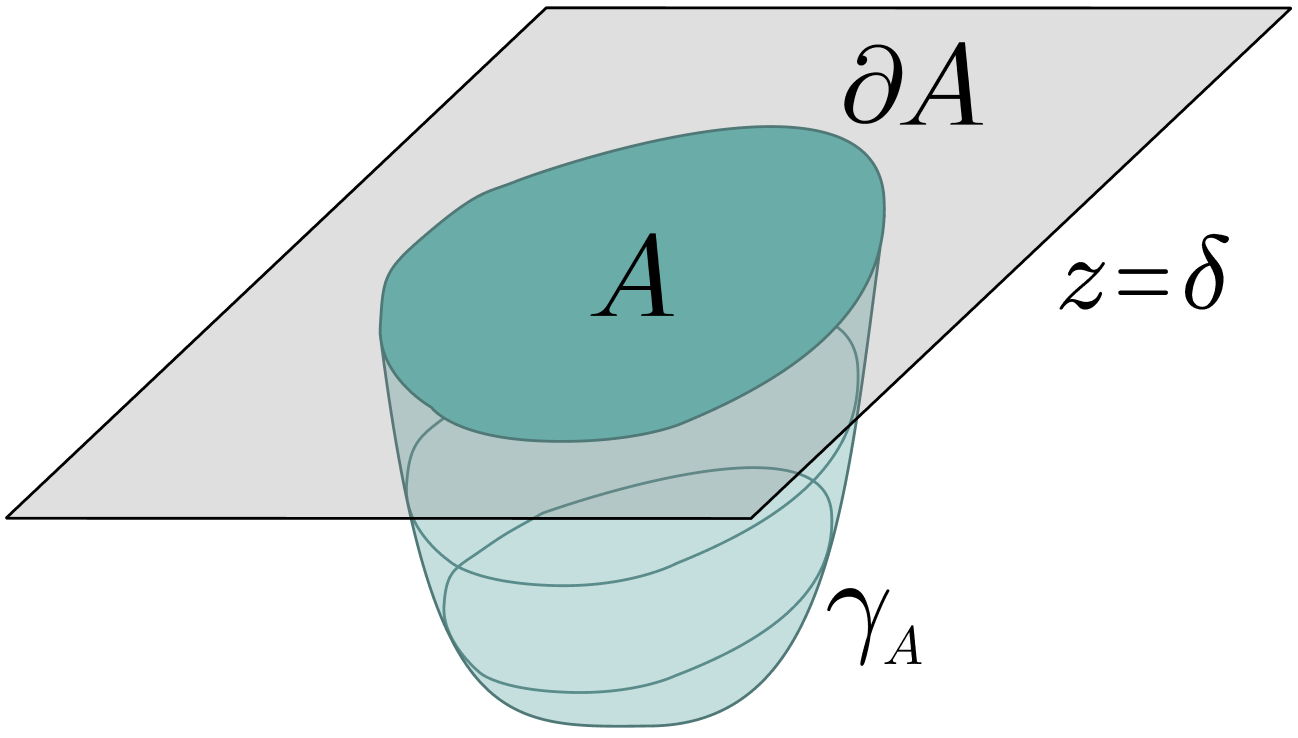
\includegraphics[width=0.25\textwidth]{../../Imatges/EE_AdS-CFT-D.png}
\caption{Regió $A$ (blau fosc) i la seva frontera $\partial A$ dins una llesca d'AdS $z=\delta$ gris) i una candidata a superfície mínima d'AdS $\gamma_A$ (blau clar).}
\label{fig:EE_AdS-CFT}
\end{wrapfigure}

La fórmula de Ryu-Takayanagi és vàlida per a sistemes genèrics i proveeix una pista de com la geometria de l'espaitemps pot emergir de mera informació quàntica.

Com es pot verificar, la fórmula de Ryu-Takayanagi per a un AdS ($d+1$)-dimensional reprodueix el comportament general esperat de l'EE (Eq.~(\ref{eq:EE_CFT})) per una CFT $d$-dimensional \cite{ryu_aspects_2006, nishioka_holographic_2009}. Anem a veure-ho explícitament.


\subsection{Entropia d'entrellaçament d'un disc en CFT\texorpdfstring{$_3$}{3}} \label{ss:EE-disk}

En aquesta secció calculem l'EE per a una regió circular en una CFT$_3$ hologràfica dual a la gravetat d'Einstein. Utilitzarem aquest càlcul per verificar l'expressió general de l'EE per a una QFT, identificant el coeficient universal per aquest tipus de teoria, i i"lustrarem com AdS ens proveeix d'un regulador ultraviolat geomètric.

Sigui $A$ una regió en forma de disc de radi $R$ definida en la frontera conforma d'un AdS$_4$ pur. Aquesta regió es defineix en coordenades polars com
$
A = \{ ( r, \theta, z, t ) \ | \ t = 0, z = \delta, r \le R \}
$.
Parametritzem la superfície del \emph{bulk} d'àrea mínima com
$
\gamma_A^\text{min} = \{ ( r, \theta, z, t ) \ | \ t = 0, z = f (r, \theta) \} 
$,
on $f(r,\theta)$ és una certa funció que necessitem identificar. No hi ha cap propietat a la teoria de l'espaitemps d'AdS que no permeti la simetria de $\partial A$ en la coordenada $\theta$ ser transferida a $\gamma_A^\text{min}$. Per tant, $z=f(r)$.
La mètrica d'AdS$_4$ es llegeix com
\eq{1Ametric}{
\mathrm{d}s^2_{\text{AdS}_4} = g_{\mu \nu} \mathrm{d}x^\mu \mathrm{d}x^\nu =
\frac{L^2}{z^2} [ -\mathrm{d}t^2 + \mathrm{d}z^2 + \mathrm{d}r^2 + r^2 \mathrm{d}\theta^2 ] \ . \nonumber
}
La mètrica induïda a la superfície $\gamma_A^\text{min}$ és al seu torn expressada com
\eq{1gammaAmetric}{
\mathrm{d}s^2_{\gamma_A^\text{min}} = h_{i j} \mathrm{d}x^i \mathrm{d}x^j =
\frac{L^2}{f(r)^2} \left[ \left( 1+ \dot{f}(r)^2 \right) \mathrm{d}r^2 + r^2 \mathrm{d}\theta^2 \right] \ , \nonumber
}
on $ \dot{f}(r) \equiv \partial f/\partial r$. El determinant de la mètrica induïda serà
$
h = L^4 r^2 ( 1 + \dot{f}(r)^2 )/f(r)^4
$.
El valor mínim de la integral sobre les coordenades polars de l'arrel quadrada de la mètrica induïda es correspondrà amb l'àrea de $\gamma_A^\text{min}$. Per tant, a través de la fórmula de Ryu-Takayanagi, l'EE corresponent a la regió $A$ serà
\eq{1EEA}{
S_A = \text{min} \int_{\gamma_A} \frac{\sqrt{h} \ \mathrm{d}x^i}{4G} = \frac{\pi L^2}{2G} \, \text{min} \int_r \mathrm{d}r \frac{r \sqrt{ 1 + \dot{f}(r)^2 }}{f(r)^2} \ ,\nonumber
}
on a la segona igualtat hem dut a terme la integral angular. La integral resultant en $r$ ha de ser avaluada en la superfície mínima. Per trobar-la, extremitzem el funcional utilitzant les equacions d'Euler-Lagrange pel Lagrangià efectiu $\calL [r,f(r),\dot{f}(r)]$. Es llegeixen com
\eqgat{1EL}{
\frac{\partial \calL}{\partial f} - \frac{\mathrm{d}}{\mathrm{d}r} \left[ \frac{\partial \calL}{\partial \dot{f}} \right] = 0 \nonumber \\
\longrightarrow \left( 1+\dot{f}^2 \right) \left( -2r-f\dot{f}-rf\ddot{f} \right) + rf\dot{f}^2\ddot{f} = 0 \ .\nonumber
}
Es pot provar que $f(r) = \sqrt{R^2 - r^2}$ és solució de la relació anterior i correspon a la funció que minimitza el funcional de l'EE i que connecta amb la regió fronterera $A$. Per tant, la superfície de mínima àrea resulta ser una mitja esfera.

Per calcular la integral de l'expressió de l'EE, primer hem de determinar els seus límits de forma curosa. L'inferior correspon a la part més baixa de la mitja esfera dins del \emph{bulk}, on $r_\text{min}=0$. El superior connecta la superfície amb la frontera conforma, és a dir, $z=\delta=\sqrt{R^2-r_\text{max}^2}$. Si no haguéssim inclòs $\delta$ i haguéssim integrat tot el camí fins a $z=0$, el resultat hauria divergit. Això és precisament el que esperem de l'EE, que divergeixi en el continu. En aquest cas, el límit geomètric introduït en la coordenada hologràfica, $z=\delta$, juga el rol del regulador ultraviolat de l'EE. El resultat final per l'EE del disc és
\eqgat{1sol}{
S_A = \frac{\pi L^2}{2G} \, \int_0^{\sqrt{R^2-\delta^2}} \mathrm{d}r \frac{r}{f(r)^2} \sqrt{ 1 + \dot{f}(r)^2 } = \nonumber \\
= \frac{\pi L^2}{2G} \frac{R}{\delta} - \frac{\pi L^2}{2G}+\mathcal{O}(\delta) \ . \nonumber
}
Coincideix amb l'expressió general per l'EE d'una CFT (Eq.~(\ref{eq:EE_CFT})) amb $d=3$. Repetint el càlcul per diverses regions i en diferents dimensions, cada estructura que es troba és sempre consistent \cite{ryu_aspects_2006,ryu_holographic_2008}.

De l'expressió anterior podem identificar la contribució universal a l'EE per a una teoria hologràfica 3-dimensional dual a la gravetat d'Einstein. El resultat es llegeix com
\eq{suniv}{
s_\text{univ} = \frac{\pi}{2} \frac{L^2}{G} \ .
}
En el cas d'una regió en forma de disc, com la que acabem de considerar, $s_\text{univ}$ està relacionada amb una altra quantitat important, concretament, l'energia lliure Euclidiana d'una esfera 3-dimensional. Tenim $s_\text{univ}= -\log Z_{\mathbb{S}^3}$ per CFTs generals \cite{casini_towards_2011}. Per tant, trobem que per teories hologràfiques duals a la gravetat d'Einstein 4-dimensional, l'energia lliure de l'esfera ve donada en termes del radi d'AdS i de la constant de Newton per l'Eq.~(\ref{eq:suniv}).


\subsection{Subadditivitat forta} \label{ss:SS}

La \emph{subadditivitat forta} és una propietat general fonamental de l'EE. Relaciona les EEs de dos regions $A$ i $B$ amb les de la seva unió $A \cup B$ i intersecció $A \cap B$ (Fig.~\ref{fig:SS}):
\eqgat{EE_strong-subadd}{
S(A) + S(B) \ge S(A \cup B) + S(A \cap B) \ .
}
\begin{wrapfigure}[13]{r}{0.25\textwidth}
\centering
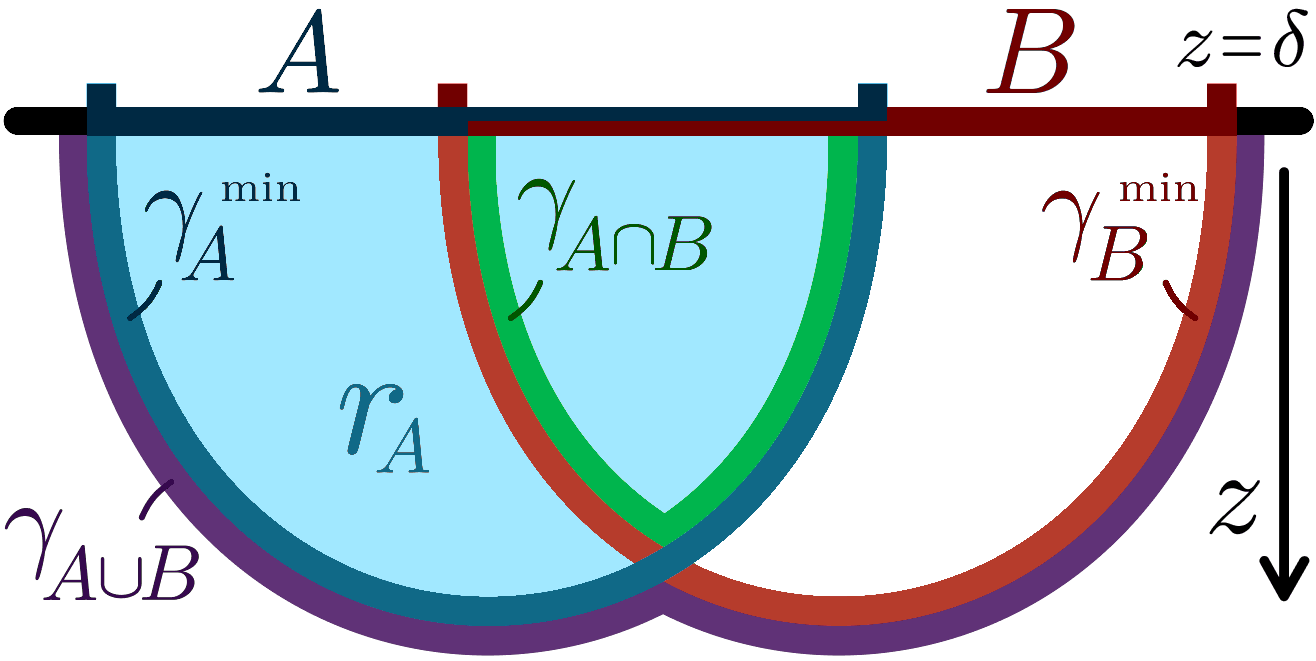
\includegraphics[width=0.25\textwidth]{../../Imatges/SS_2-D.png}
\caption{Representació de les superfícies $\gamma_A^\text{min}$ i $\gamma_B^\text{min}$, la seva unió $\gamma_{A \cup B}$ i intersecció $\gamma_{A \cap B}$, i la regió del \emph{bulk} $r_A$.}
\label{fig:SS}
\end{wrapfigure}
Aquesta desigualtat és completa per qualsevol teoria de mecànica quàntica, però és notablement difícil de provar en general. Un test important de la validesa de la fórmula de Ryu-Takayanagi serà si la compleix. Resulta ser particularment fàcil de provar que ho fa \cite{headrick_holographic_2007}.

Definim $r_A$ i $r_B$ com les regions del \emph{bulk} dins de $\gamma^{\text{min}}_A$ i $\gamma^{\text{min}}_B$, respectivament. La seva unió i intersecció serà $r_{A \cup B} \equiv r_A \cup r_B$ i $r_{A \cap B} \equiv r_A \cap r_B$. Les fronteres d'aquestes regions es poden descompondre com
\eq{SS_dr-1}{
\partial r_{A \cup B} = (A \cup B) \cup \gamma_{A \cup B} \ , \ \partial r_{A \cap B } = (A \cap B) \cup \gamma_{A \cap B} \ , \nonumber
}
on $\gamma_{A \cup B}$ i $\gamma_{A \cap B}$ són els segments dins del \emph{bulk} de les superfícies frontereres de $r_{A \cup B}$ i $r_{A \cap B}$. Aquestes superfícies estan connectades a $\partial (A \cup B)$ i $\partial (A \cap B)$, respectivament, però res ens diu que hagin de ser les corresponents superfícies d'àrea mínima $\gamma^{\text{min}}_{A \cup B}$ i $\gamma^{\text{min}}_{A \cap B}$. Les àrees de $\gamma_{A \cup B}$ i $\gamma_{A \cap B}$ corresponen a límits superiors de les possibles àrees mínimes. A més, observem de forma trivial que la suma de les àrees de $\gamma_{A \cup B}$ i $\gamma_{A \cap B}$ és igual a la suma d'àrees de $\gamma^{\text{min}}_A$ i $\gamma^{\text{min}}_B$. Per tant,
\eq{SS_gamma-1}{
{\text{Area}}(\gamma^{\text{min}}_A) + {\text{Area}}(\gamma^{\text{min}}_B) \ge {\text{Area}}(\gamma^{\text{min}}_{A \cup B}) + {\text{Area}}(\gamma^{\text{min}}_{A \cap B}) \ . \nonumber
}
Llavors, la fórmula de Ryu-Takayanagi (Eq.~(\ref{eq:EE_RT})) implementa la propietat de subadditivitat forta d'una forma geomètrica simple que utilitza el principi de minimització de les superfícies hologràfiques d'AdS.


\subsection{Correccions a la fórmula de Ryu-Takayanagi} \label{ss:EE_HO}

La fórmula de Ryu-Takayanagi proveeix l'EE per a teories hologràfiques duals a la gravetat d'Einstein en dimensions generals. En canvi, la descripció Einsteiniana s'ensorra si ens movem lluny del règim de fort acoblament i alt nombre de colors. Per la banda gravitacional, això es manifesta amb l'aparició de correccions tant cordoses com quàntiques.

Les correccions cordoses apareixen com termes de curvatura superior en l'acció gravitatòria. Això produeix correccions a la fórmula de l'àrea de Ryu-Takayanagi de forma similar a com la fórmula de Bekenstein-Hawking per l'entropia d'un forat negre (Eq.~(\ref{eq:BH})) se substitueix per la fórmula de Wald \cite{iyer_properties_1994} en presència de correccions de curvatura superior. No obstant això, substituir el funcional de l'EE pel de Wald no funciona de forma general. Esquemàticament, la fórmula sencera és \cite{dong_holographic_2014}
\begin{equation}\label{hee}
S_A=S_{\text{Wald}}+ S_{\text{Anomaly}} \ ,
\end{equation}
on $S_{\text{Wald}}$ es redueix en la de Ryu-Takayanagi en el cas de gravetat d'Einstein. Si no, conté termes que involucren diverses components del tensor de Riemann. $S_{\text{Anomaly}}$ simplement es desvaneix per gravetat d'Einstein, però inclou termes que involucren curvatures extrínseques de la superfície mínima generalitzada per teories més generals.

També es poden considerar correccions quàntiques a la fórmula de Ryu-Takayanagi relacionades amb efectes de mecànica quàntica en el \emph{bulk}. Aquestes correccions quàntiques venen donades bàsicament per l'EE de camps quàntics que viuen dins de la regió del \emph{bulk} dins de la superfície de mínima àrea, $r_A$ ---veure Fig.~\ref{fig:SS}. La fórmula corregida es llegeix \cite{faulkner_quantum_2013}
\eq{EEquantum}{
S_A = \frac{\text{Area} (\gamma_A^\text{min})}{4 G} + S_{r_A} + \calO(G) \ ,
}
on la correcció $S_{r_A}$ és d'ordre $\calO(G^0)$ i també hi hem inclòs una possible correcció subjacent.


\vspace{-0.4cm}
\section{Conclusions} \label{s:Conclusions}

Hem explorat diversos aspectes de la fórmula de Ryu-Takayanagi ---un resum dels resultats presentats es pot trobar a la introducció. És una entrada excepcional en el diccionari hologràfic que ens permet calcular una propietat genuïnament quàntica com l'EE de regions frontereres, en termes d'una quantitat completament clàssica relacionada amb la geometria de l'espaitemps, específicament, l'àrea de superfícies extremals dins d'AdS.

La connexió entre la geometria de l'espaitemps i l'entrellaçament es pot fer més explícita. Sorprenentment, es pot veure que la primera llei de l'EE implica, per CFTs hologràfiques, que pertorbacions de la mètrica del \emph{bulk} satisfan les equacions d'Einstein linealitzades \cite{faulkner_gravitation_2014}. En certa forma, l'estructura d'entrellaçament de la teoria a la frontera controla la dinàmica del camp gravitatori, que llavors esdevé un fenomen emergent.


\begin{acknowledgments}

    M'agradaria expressar el meu sincer agraïment al professor Pablo Bueno per la seva orientació i experiència. També vull donar les gràcies a la meva família i amics pel seu suport i paciència.
    
\end{acknowledgments}



\bibliography{TFG_CAT.bib}
% \bibliographystyle{abbrv}


\end{document}